\section{On-demand evaluation for KBP}
\label{sec:kbpo:application}
Applying the on-demand evaluation framework to a task requires us to answer three questions:
\begin{enumerate}
    \itemsep0pt
  \item What is the desired distribution over system predictions $p_i$?
  \item How do we label an instance $x$, i.e.\ check if $x \in \sY$?
  \item How do we sample from the unknown set of true instances $x \sim p_0$?
\end{enumerate}
In this section, we present practical implementations for knowledge base population.

\subsection{Sampling from system predictions}
% 1. what is the point of this distribution?
% - prevent over sampling instances.
%\ac{@PL:\@ I think that the role of $p_i$ is really very subtle, but very important. I hope the below paragraph highlights the paradigm shift in how one has to think about on-demand evaluation.}
Both the official TAC-KBP evaluation and the on-demand evaluation we propose use micro-averaged precision and recall as metrics. However, in the official evaluation, these metrics are computed over a fixed set of evaluation entities chosen by LDC annotators, resulting in two problems: (a) defining evaluation entities requires human intervention and (b) typically a large source of variability in evaluation scores comes from not having enough evaluation entities (see e.g.\ \citep{webber2010measurement}). In our methodology, we replace manually chosen evaluation entities by sampling entities from each system’s output according $p_i$. In effect, $p_i$ makes explicit the decision process of the annotator who chooses evaluation entities.

%\ac{@PL:\@ This paragraph goes into details, but I felt that it was useful to illustrate how we tailored a distribution to meet our evaluation goals.}
Identifying a reasonable distribution $p_i$ is an important implementation decision that depends on what one wishes to evaluate.
Our goal for the on-demand evaluation service we have implemented is to ensure that KBP systems are fairly evaluated on diverse subjects and predicates, while at the same time, ensuring that entities with multiple relations are represented to measure completeness of knowledge base entries.
As a result, we propose a distribution that is inversely proportional to the frequency of the subject and predicate and is proportional to the number of unique relations identified for an entity (to measure knowledge base completeness).
%See \refapp{implementation} in the supplementary material for an analysis of this distribution and a study of other potential choices.

%Recall that a KBP system predicts a set of relation instances of the form (\entity{subject}, \relation{predicate}, \entity{object}, \textsc{provenance}).
%Simply choosing $p_i$ to be the uniform distribution over this set causes our evaluation metrics to be be dominated by a few common predicates (e.g.\ professional titles) or subject entities (e.g.\ ``United States of America'').
%Instead, we propose the following distribution which we reasonably approximates our goals:\footnote{
%See \refapp{implementation} for an analysis of this distribution and a study of other potential choices.} 
%\begin{align*}
%  p_i(x) &\eqdef \frac{\operatorname{\#uniq-relns}_i(x)}{\operatorname{\#pred-insts}_i(x) \operatorname{\#subj-insts}_i(x)},
%\end{align*}
%where $\operatorname{\#uniq-relns}_i(x)$ measures the number of unique relations (\entity{subject}, \relation{predicate}, \entity{object} triples) with the same \entity{subject} as $x$ in the system's output $X_i$, 
%$\operatorname{\#pred-insts}_i(x)$ measures the number of instances with the same \relation{predicate} as $x$ in $X_i$ and 
%$\operatorname{\#subj-insts}_i(x)$ measures the number of instances with the same \relation{subject} as $x$ in $X_i$.

%%The choice of distribution over this set determines how much we put weight on rare predicates and subject entities in our evaluation metric. % in our precision score. % PL: for recall 
%We therefore propose two instance distributions that evaluate precision and recall scores macro-averaged over predicates and subject entities, respectively:
%\begin{align*}
%  p_i^\text{(pred)}(x) &\eqdef \frac{1}{\operatorname{\#preds}(X_i)} \frac{1}{\operatorname{\#insts}(X_i, \relation{pred}(x))} \\
%  p_i^\text{(subj)}(x) &\eqdef \frac{1}{\operatorname{\#subjs}(X_i)} \frac{1}{\operatorname{\#insts}(X_i, \relation{subj}(x))}
%\end{align*}
%where $\operatorname{\#preds}$, $\operatorname{\#nsubjs}$ specifies the number of predicates, subject entities in $X_i$ respectively and $\operatorname{\#insts}$ the number of instances with the given predicate or subject entity.
%See \refapp{implementation} for more details.
\begin{figure}[!th]
  \centering
  \begin{subfigure}{\textwidth}
  \centering
    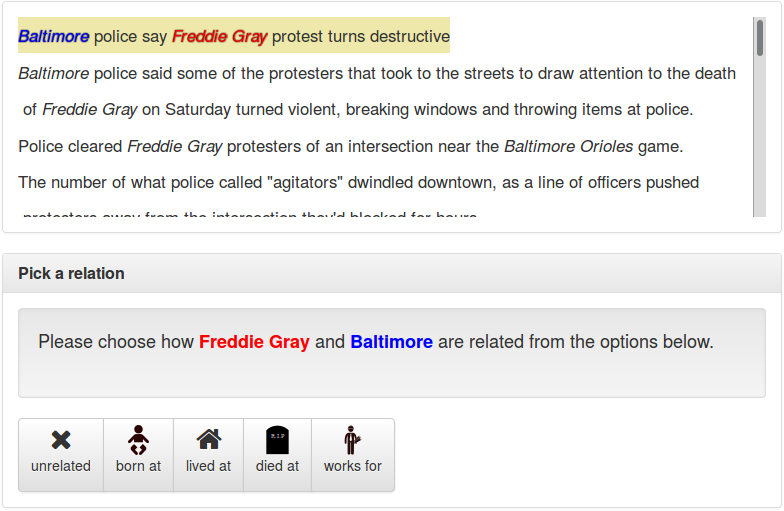
\includegraphics[width=0.9\textwidth]{figures/interface/relation-interface}
    \caption{\label{fig:kbpo:relation-interface}}
  \end{subfigure}

  \begin{subfigure}{\textwidth}
  \centering
    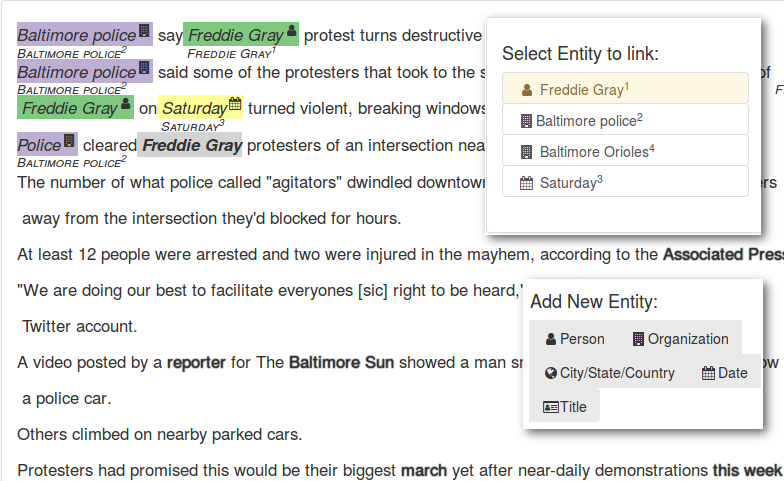
\includegraphics[width=0.9\textwidth]{figures/interface/extraction-interface}
    \caption{\label{fig:kbpo:entity-interface}}
  \end{subfigure}

  \caption[Annotation interfaces for KBP]{\label{fig:kbpo:interfaces}
  Interfaces for annotating (a) relations and (b) entities.
  }
\end{figure}

\subsection{Labeling predicted instances}
We label predicted relation instances by presenting the instance's provenance to crowdworkers
  and asking them to identify if a relation holds between the identified subject and object mentions (\reffig{kbpo:relation-interface}). 
  Crowdworkers are also asked to link the subject and object mentions to their canonical mentions within the document and to pages on Wikipedia, if possible, for entity linking.
On average, we find that crowdworkers are able to perform this task in about 20 seconds, corresponding to about \$0.05 per instance.
We requested 5 crowdworkers to annotate a small set of 200 relation instances from the 2015 TAC-KBP corpus 
and measured a substantial inter-annotator agreement with a Fleiss' kappa of 0.61 with 3 crowdworkers and 0.62 with 5. % \pl{why does it go up with more annotators?}.
%On manually inspection of these instances, we observed a precision of about 75\%.
%While this precision is slightly less than the 80\% obtained by annotators at LDC \citep{ellis2016overview}, we believe it could be easily improved with appropriate changes to the annotation interface.
Consequently, we take a majority vote over 3 workers in subsequent experiments.
%leading to a total cost of \$0.15 per relation instance.

%\pl{what does it mean to annotate a relation - get all the relation instances for that relation or just one?}.
\subsection{Sampling true instances}
Sampling from the set of true instances $\sY$ is difficult because we can't even enumerate the elements of $\sY$.
As a proxy, we assume that relations are identically distributed across documents and have crowdworkers annotate a random subset of documents for relations using an interface we developed (\reffig{kbpo:entity-interface}).
Crowdworkers begin by identifying every mention span in a document.
  For each mention, they are asked to identify its type, canonical mention within the document
  and associated Wikipedia page if possible.
They are then presented with a separate interface to label predicates between pairs of mentions within a sentence that were identified earlier.

We compare crowdsourced annotations against those of expert annotators using data from the TAC KBP 2015 EDL task on 10 randomly chosen documents.
We find that 3 crowdworkers together identify 92\% of the entity spans identified by expert annotators, while 7 crowdworkers together identify 96\%.
When using a token-level majority vote to identify entities, 3 crowdworkers identify about 78\% of the entity spans; this number does not change significantly with additional crowdworkers.
We also measure substantial token-level inter-annotator agreement using Fleiss' kappa for identifying typed mention spans ($\kappa = 0.83$), canonical mentions ($\kappa = 0.75$) and entity links ($\kappa = 0.75$) with just three workers.
Based on this analysis, we use token-level majority over 3 workers in subsequent experiments.
%We also manually labeled 200 relation instances that from the exhaustively annotated documents and observed a precision of about 75\%.
%While this precision is slightly less than the 80\% obtained by annotators at LDC \citep{ellis2016overview}, we believe it could be easily improved with appropriate changes to the annotation interface.

The entity annotation interface is far more involved and takes on average about 13 minutes per document, corresponding to about \$2.60 per document, while the relation annotation interface takes on average about \$2.25 per document.
Because documents vary significantly in length and complexity, we set rewards for each document based on the number of tokens (.75c per token) and mention pairs (5c per pair) respectively.
With 3 workers per document, we paid about \$15 per document on average.
Each document contained an average 9.2 relations, resulting in a cost of about \$1.61 per relation instance.
We note that this is about ten times as much as labeling a relation instance.

%We defer details regarding how documents themselves should be weighted to capture diverse entities that span documents to \refapp{implementation}.
%We provide details regarding our sampling scheme and its distribution over entities in \refapp{implementation} of the supplementary material.
%When considering uniformly sampled documents, we found that a majority of the relations extracted correspond to very rare entities and result in very few entities with more than one relation (\reffig{entity-distribution}).
%In contrast, the TAC KBP query are almost evenly split between rare and semi-frequent entities.
%As a heuristic, we adopt the following two-stage sampling procedure:
%First, 20\% of our exhaustive document collection is sampled uniformly and annotated.
%We then uniformly sample the entities annotated to create a collection of ``evaluation entities''.
%Finally, we construct the remaining 80\% of our document collection by searching for documents that contain the evaluation entities according to an exact string match. This process results in far more entities of medium frequency.
